\subsubsection{Vorstellung des ESP8266 Lua}        
\label{sec:Vorstellung des ESP8266} 

Der ESP8266 Lua ist ein Entwicklungsboard, welches bereits ein integriertes WLAN Modul besitzt und mit einem \ac{TCP}/\ac{IP} Stack ausgestattet ist. Einer der vorgesehenen Einsatzzwecke ist unter anderem das \ac{IoT}. Das Board kann zudem mit Steckbrettern arbeiten und bietet daher ähnliche Möglichkeiten, wie das bereits erwähnte \nameref{sec:Pretzelboard-1}. 

Zudem ist es möglich, dass die Software für das ESP8266 Lua Entwicklungsboard ebenfalls über die Arduino \ac{IDE} entwickelt werden kann. Allerdings sind technische Unterschiede zum Pretzelboard vorhanden, was dazu führt, dass andere Treiber genutzt werden müssen. 
Diese können nachinstalliert werden und stehen dann zur Nutzung des Boards bereit. (vgl. \cite{Carius.15.01.2017}\cite{.d})

\begin{figure}[!htb]
	\centering
	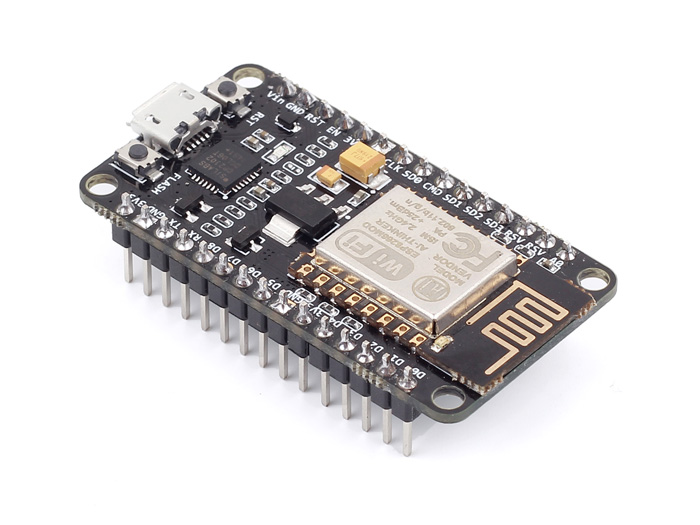
\includegraphics[scale=0.4]{ESP.jpg}
	\caption[ESP8266]{ESP8266,\\ Quelle: https://www.roboter-bausatz.de/media/image/dc/14/6e/113990105-1.jpg}
\end{figure}

\subsubsection{Verwendung im Projekt}        
\label{sec:Verwendung des ESP8266} 
Das Board wird im Rahmen des Projektes als weiterer Button genutzt. Es bietet sich für diese Funktion an, da es ebenfalls recht klein ist und alle benötigten Funktionen bereits vorhanden sind. Neben den vorhandenen Funktionen ist auch die Möglichkeit vorhanden, dass eine bereits durch das Bretzelboard bekannte Entwicklungsumgebung genutzt werden kann. Das bietet die Möglichkeit, dass statt des \ac{UDP} Protokolls das bereits erwähnte \ac{TCP} (vgl. Kapitel \ref{sec:TCP-1}) Protokoll ausprobiert werden kann. 

Der Aufbau des Boards soll ebenfalls durch ein Elektroniksteckboard umgesetzt werden. Dazu wird das Board auf eben dieses Steckboard gesetzt und mit einem Button, Statusleuchten und entsprechenden Kabeln verbunden. Nach der Betätigung des Buttons wird das Board geweckt und eine Funktion schickt ein entsprechendes Datenpaket an einen Empfänger.
\begin{figure}[!htb]
	\centering
	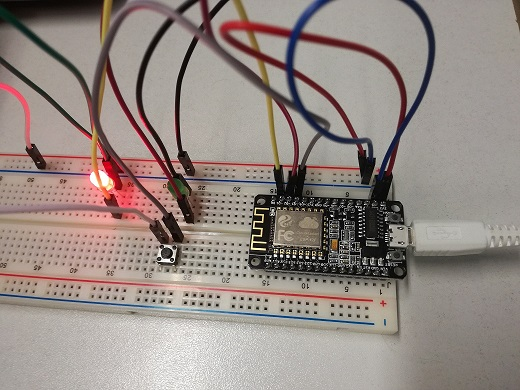
\includegraphics[scale=0.5]{ESP_Projekt.jpg}
	\caption[ESP8266 im Projekt]{ESP8266 im Projekt,\\ Quelle: Eigene Aufnahme}
\end{figure}
\newpage


 
